\documentclass{article}
\usepackage[margin=3cm]{geometry}
\usepackage{textcomp}
\usepackage{graphicx}
\usepackage{float}
\usepackage{amsmath}
\usepackage[hidelinks]{hyperref}
\urlstyle{same}

\title{When normalization gets prickly: are spike-ins good enough for single-cell RNA sequencing data?}
\author{Aaron Lun}

\begin{document}

\maketitle

\section{Introduction}
Single-cell RNA sequencing (scRNA-seq) is a powerful technique for studying transcriptional activity in individual cells.
Briefly, RNA is isolated from single cells, converted into cDNA and sequenced using massively parallel sequencing technologies \cite{shapiro2013singlecell}.
This can be done on microfluidics platforms or with protocols such as Smart-seq2 \cite{picelli2014full} that use microtiter plates.
Gene expression can be quantified by mapping the read sequences to the genome and counting the number of reads mapped to each gene.
To avoid amplification biases, individual transcript molecules can be tagged with unique molecular identifiers (UMIs) \cite{islam2014quantitative}, such that sequencing to saturation and counting UMIs will yield the number of transcripts of each gene in a cell.
%However, sequencing to saturation may not be economically feasible for hundreds or thousands of cells.
However, not all molecules will be captured and sequenced due to cell-specific inefficiencies in reverse transcription \cite{stegle2015computational}.
The presence of these cell-specific biases compromises the use of the read/UMI count as a quantitative measure of gene expression.
Some normalization is necessary to remove these biases before counts can be meaningfully compared between cells.

One commonly used normalization strategy is to use a set of genes that have constant expression across cells.
This set can consist of pre-defined ``house-keeping'' genes, or it can be empirically defined under the assumption that most genes are not differentially expressed (DE) between cells.
Counts are scaled to eliminate (presumably artifactual) differences in the coverage of this set across cells.
This removes spurious differences like those caused by composition bias, i.e., where greater sequencing of upregulated transcripts proportionally reduces the sequencing of all other genes \cite{robinson2010tmm}.
The scaled counts can then be compared between cells in downstream analyses.
This gene-based approach works well for bulk sequencing experiments where the population-wide gene expression profile is stable.
However, it may not be suitable for single-cell experiments where technical noise and biological heterogeneity complicate the identification of a reliable non-DE set. 
For example, house-keeping genes may be turned on or off by transcriptional bursting \cite{marinov2014singlecell}, while cell cycling and other processes may trigger large-scale changes in the transcriptional programme that preclude the assumption of a non-DE majority.

An alternative normalization strategy involves the use of spike-in RNA for which the identity and quantity of all transcripts is known \cite{stegle2015computational}.
The same amount of spike-in RNA is added to each cell, and the spike-in transcripts are processed along with their endogenous counterparts into a library for sequencing.
This yields a set of read (or UMI) counts for both endogenous and spike-in transcripts in each cell.
Normalization is performed by scaling the counts for each cell such that the counts for the spike-in genes are, on average, the same between cells.
The central assumption of this approach is that the same amount of spike-in RNA is added to each cell.
Thus, any differences in the coverage of the spike-in genes between cells must be artifactual in origin and should be removed by scaling.

The use of spike-ins for normalization seems preferable to the non-DE approach as it avoids making strong assumptions about the biology of single cells.
However, a major criticism of spike-ins in bulk experiments is that the same volume of spike-in RNA cannot be consistently added to each sample \cite{robinson2010tmm}.
Variable addition of spike-ins would violate the assumption of equal spike-in quantities per cell, compromising the effectiveness of normalization \cite{risso2014normalization}.
Another criticism is that synthetic spike-in transcripts may not behave in the same manner as endogenous transcripts \cite{grun2015design}.
Any cell-specific biases in capture efficiency for the latter may not be captured by the former, rendering normalization inaccurate.

The aforementioned issues with normalization are equally applicable to both plate- and microfluidics-based protocols.
Microfluidics platforms such as the Fluidigm C1 \cite{pollen2014lowcoverage} attempt to mitigate the effect of cell-specific biases by tightly controlling the reaction conditions during cDNA generation.
This is not without its own complications -- the C1 chips must be matched to the cell size, and cell capture is susceptible to doublet formation (where two cells are processed into a single library) \cite{fluidigm2016white}.
In contrast, plate-based protocols tend to be cheaper to run and are compatible with existing laboratory techniques such as indexed fluorescently-activated cell sorting (FACS).
Thus, we focus on normalization of data from plate-based protocols, to reflect their increasing use in single-cell studies (CITE BIG GUYS).

In this paper, we conduct a series of experiments to estimate the reliability of spike-in normalization in single-cell transcriptome studies employing plate-based protocols.
We use mixtures of two distinct spike-in RNA sets to quantify the variance of the added spike-in volume across cells.
We also estimate the variability in differential behaviour between the sets, to determine how cell-specific biases change between different RNA populations.
Both factors are quantitatively negligible and have only minor effects on the results of downstream analyses such as detection of DE and highly variable genes.
These results suggest that spike-ins can be safely used for routine normalization of scRNA-seq data.

% The advantage of spike-ins is that it can capture cell size and doesn't require a non-DE majority.
% However, is the cell size interesting, or should it be normalized out (in which case accurate spike-in addition wouldn't be required at all)?
% It's most obviously useful for cell cycle considerations -- possibly also cancer and in some aspects of differentiation.
% The Islam non-UMI dataset is one example where there seems to be a 20-50-fold increase in counts in the MEFs vs mESCs.
% 
% I guess spike-in normalization is more technically correct, even if you end up getting every gene as being DE (technically true in terms of molecules, but possibly irrelevant).
% Rankings definitely change - spike-in normalization would favour genes that are upregulated on top of an increase in RNA content (as these would be hugely significant).
% Standard normalization would have no preference as you seek the balance between the two extremes.
% On the other hand, any non-DE genes with no change in the molecule number will be called as significant in standard normalization, which is definitively wrong.
% You could have your cake and eat it by separating the DE list into up/down changes for easier examination of the up/down changes.

\section{Results}

\subsection{Overview of the mixture experiments}
We used two spike-in sets -- the External RNA Controls Consortium (ERCC) set and the Spike-in RNA Variants (SIRV) set.
Equal volumes of each spike-in set were added into a well and converted into a library with the Smart-seq2 protocol.
This process was repeated for multiple wells, and sequencing was performed on all of the generated libraries.
For each library, reads were mapped back to the genome and counted into genes.
The total count across all genes was computed for each spike-in set, and the log-ratio of the total counts between the two sets was calculated (denoted here as $\theta_i$).
The variance of this log-ratio across wells contains the variance in the addition of each spike-in volume $\sigma_{vol}^2$;
    variance in the difference in behaviour between spike-in sets, where $\psi_i$ represents the fold change in the capture efficiency between sets;
    and additional technical variability from library preparation and sequencing $\sigma^2_{lib(s)}$.
In other words, for $s=1$ (ERCC) and 2 (SIRV), the variance of $\theta_i$ can be decomposed to 
\[
    \mbox{var}(\theta_i) = 2\sigma_{vol}^2 + \sigma^2_{lib(1)} + \sigma^2_{lib(2)} + \mbox{var}(\log \psi_i) \;.
\]

The experiment was repeated after mixing the two spike-in sets before addition into each well. 
The variance of the log-ratio of the total counts of the two spike-in sets was then computed across wells (denoted here as $\theta_i'$).
Here, the ratio of the added volumes of two spike-in sets is constant across all wells.
This means that variability in volume addition will not contribute to variability of $\theta_i'$, i.e.,
\[
    \mbox{var}(\theta_i') = \sigma^2_{lib(1)} + \sigma^2_{lib(2)} + \mbox{var}(\log \psi_i) \;.
\]
Subtracting the estimated variance from that of the first experiment yields an estimate of $\sigma_{vol}^2$.

The variance of $\psi_i$ is relevant as it determines the effect of differences in behaviour between different RNA populations.
If the relative capture efficiency of spike-in to endogenous transcripts was the same (non-unity) value in all wells, it would have no effect on relative quantification of gene expression, as the difference in behaviour would cancel out when normalized expression values are compared between cells.
However, if the relative efficiency varies across cells, cancellation would not occur such that cell-specific biases would affect the comparison between cells.
To estimate $\mbox{var}(\psi_i)$, further decomposition of $\mbox{var}(\theta_i')$ can be achieved by considering the variance of the log-ratios between transcripts in the same spike-in set.
The assumption is that, on average, different transcripts from the same set will have the same capture efficiency.
If one were to split the set into two halves and compute the log-ratio between them, the variance of those log-ratios would not contain any contribution from the variance in the fold change in efficiency (as this should be equal to unity for all wells).
Instead, any variance should consist solely of the additional technical variability $\sigma^2_{lib(s)}$.
This can be used to estimate $ \sigma^2_{lib(1)}$ and $\sigma^2_{lib(2)}$, both of which can then be subtracted from $\mbox{var}(\theta_i')$ to yield an estimate of $\mbox{var}(\log \psi_i)$.

Both experiments were performed with a cell in each well, sourced from a homogeneous cell line.
The log-ratio between spike-in and cellular counts was computed for each well.
The variance of this log-ratio across wells includes the biological variability in total RNA across cells.
This serves as a reference to which the spike-in-based components of the technical variability can be compared. 

A schematic of the experimental design is provided in Figure~\ref{fig:expdesign}.
The mathematical framework underlying the variance decomposition is described in Section~1 of the Supplementary Materials.

% It should be stressed that the specific choice of population does not matter.
% Once the variance is estimated, it can be applied to other studies involving different RNA populations.

\begin{figure}[H]
\begin{center}
\includegraphics[width=\textwidth]{pics/plate_setup.pdf}
\end{center}
\caption{Schematic of the experimental design to assess the variability of spike-ins in a plate-based scRNA-seq protocol.
The first experiment (A) involves adding an equal volume of each spike-in set into each well during the reverse transcription (RT) step.
The second experiment (B) involves adding an equal volume of a pooled mixture of the two spike-ins into each well, again during the RT step (done twice for consistency).
Sequencing is performed and the log-ratio of the total count between spike-in sets is computed for each well.
Components of the spike-in variability can be separated by estimating the variance of the log-ratios across wells and comparing the estimates between experiments.
}
\label{fig:expdesign}
\end{figure}

\subsection{Variability in spike-in addition or efficiency is negligible}
% Mention switched order.
% No effect of different cell treatments.
% Same total count for spike-ins between premixed and not premixed.
% Normality.

\subsection{Assessing the downstream effect of variability with simulations}
We assessed whether the results of downstream analyses were sensitive to spike-in variability, especially for those analyses that depend on the assumption of constant spike-ins for normalization.
Simulations were prepared from real data sets containing counts for spike-in transcripts.
Specifically, the added volume and relative capture efficiency of spike-ins for each well were resampled and the spike-in counts were rescaled to reflect this new volume/efficiency.
The results of the analysis on the simulated data were then compared to the original results.
Any changes indicate that the analysis is sensitive to spike-in variability.
The advantage of this approach is that it only modifies the scale of the spike-in counts -- the counts for the cellular genes are used directly and do not need to be simulated.
The variance of the sampling distribution for the volume/efficiency is also based on the experimental estimates of spike-in variance.
This ensures that sensitivity will be assessed under realistic conditions. 

\section{Discussion}

\section{Methods}

\subsection{Spike-in mixture experiments with Smart-seq2}
% On a single plate, so no plate effects.

\subsection{Data analysis for the mixture experiments}
Reads were mapped to the mm10 build of the mouse genome with additional sequences for transcripts in the ERCC (\url{https://tools.thermofisher.com/content/sfs/manuals/ERCC92.zip}) and SIRV (\url{https://www.lexogen.com/wp-content/uploads/2015/11/SIRV_Sequences_151124.zip}) spike-in sets.
Mapping was performed using the subread aligner v1.5.0 \cite{liao2013subread} in single-end RNA-seq mode with only unique alignments being retained.
Reads with mapping qualities greater than or equal to 10 were counted into exonic regions of genes using the featureCounts function in the Rsubread package v1.20.1 \cite{liao2014featurecounts}.
This was performed using the NCBI GRCm38 mouse annotation along with the annotation for the ERCC and SIRV transcripts, to obtain a count for each endogenous and spike-in gene in each well.

In each well, the sum of counts across all transcripts in each spike-in set was computed.
The log$_2$-ratio between the count sums of the ERCC and SIRV sets was calculated.
To estimate $\mbox{var}(\theta_i)$, a linear model was fitted to the log-ratios for all wells where the two spike-in sets were added separately.
This used a one-way layout where each combination of treatment (control or oncogene-induced) and spike-in addition order (ERCC or SIRV first) was treated as a separate group.
The variance was estimated as the mean of the squared residual effects.
This was repeated for $\mbox{var}(\theta_i')$ using all wells where premixed spike-ins were added.
Here, the model only contained two groups as addition order was irrelevant.

Variance decomposition was performed as described in Section~1 of the Supplementary Materials using the above estimates.
To determine the variability of $\psi_i$, each spike-in set was partitioned into two roughly similar halves.
This was done by sorting all transcripts in each set by their average counts; assigning all odd-ranked transcripts to one half; and assigning the remaining transcripts to the other half.
The log-ratios between the sums of the two halves were then used to estimate $\mbox{var}(\log \psi_i)$.

\subsection{Simulation design for resampling spike-in variability}
For each data set, the sum of the spike-in counts (referred to here as the spike-in total) was computed for each cell.
The variance of the log$_2$-transformed spike-in totals across cells includes sampling noise during library preparation or sequencing, variability in sequencing depth, and the variance of spike-in addition and capture efficiency between wells.
The final component (denoted here as $s^2$) represents spike-in variability and must be removed prior to simulation.
Otherwise, resampling will introduce variance for addition/efficiency on top of what is already present, leading to overrepresentation of $s^2$ in the variance of the simulated totals.
Removal was achieved by scaling the log$_2$-totals such that the variance across wells was reduced by $s^2$ without changing the mean.
The scaled log-values were then transformed back to ``processed'' totals that contain no variability due to addition or behaviour.

Simulations were performed by sampling a new value for the combined addition/efficiency effect in each cell.
Specifically, the effect for each cell was sampled independently from a $2^X$ distribution where $X \sim \mbox{Normal}(0, s^2)$.
This was used to scale the processed total to obtain a simulated total for each cell.
Counts for individual spike-in transcripts were then scaled to reflect this new total in each cell.
In this manner, the variance due to addition or capture efficiency was re-incorporated into the variance of the simulated totals across cells.
Note that addition and efficiency do not have to be simulated separately as they have the same effects in this framework -- a decrease in the spike-in total due to a decrease in the added spike-in volume cannot be distinguished from that due to reduced capture efficiency.

To scale the counts, a quantile adjustment approach was used to preserve the empirical mean-variance relationship.
A generalized linear model (GLM) was fitted to the counts across all cells for each spike-in gene, using the mglmOneGroup function in edgeR \cite{mccarthy2012differential, robinson2010edgeR} with an all-intercept design matrix.
An abundance-dependent trend was also fitted to the NB dispersions across all spike-in genes using the estimateDisp function.
In both cases, the original (natural) log-totals were used as the offsets for all cells.
The fitted GLM value and dispersion for each gene were treated as the true parameters of the NB distribution used to sample the observed count in each cell.
The simulated mean count for each gene in each cell was computed by taking the exponential of the sum of the log-simulated total for that cell and the GLM coefficient for that gene.
This was used as the mean of a simulated NB distribution, using the same value for the dispersion.
The quantile of each original count in its true distribution was mapped to a quantile in the simulated distribution, using the q2qnbinom function \cite{robinson2008small}.
This new quantile was used as the simulated count for the corresponding gene and cell.

% For simplicity, we assume that sequencing is performed to saturation in each data set, e.g., like UMIs.
% Thus, variability in the added volume will directly translate to variability in the total spike-in count.
% It also means that we do not have to rescale the cellular counts to reflect variable undersampling.
% Doing so would be problematic, as direct scaling of the counts would distort the empirical mean-variance relationship of the count data.

% The estimation of the true parameters conditions on the observed spike-in totals, and doesn't make the assumption that spike-in totals are constant.
% For example, if it turned out that you added half the amount of spike-in to one well, it wouldn't distort the estimation of the (conditional) mean.
% Okay, maybe the trended dispersion would be a bit weird, because technical variability should depend on the amount of RNA, but some inaccuracy there is forgivable.

The value of $s^2$ was set based on the previously estimated value for $\sigma^2_{vol} + \mbox{var}(\log \psi_{i}) \approx 0.05$.
This ensures that a realistic variance is used when sampling spike-in volume and efficiency in each well.

\subsection{Implementation of downstream analyses}
For the DE analyses, two scRNA-seq data sets were obtained -- one from a study with mouse embryonic stem cells (mESCs) and fibroblasts \cite{islam2011characterization} and another from a study with root epidermal and root center \textit{Arabidopsis Thaliana} cells \cite{brennecke2013accounting}.
In each study, DE genes were detected between cell types using edgeR \cite{robinson2010edgeR,lund2012detecting} and monocle \cite{trapnell2014dynamics}.
The former represents methods designed for analyses of bulk RNA-seq data, while the latter represents specialized single-cell methods.
For each method, spike-in normalization was performed by scaling the counts such that the spike-in totals were the same between cells.
The set of DE genes in the original data was then identified at a FDR of 5\% (see Section~Y in the Supplementary Materials for implementation details of each method).
This was repeated for the simulated data, and the proportion of genes common to both the original and simulated sets was computed.
The proportion of common genes in the top set of 20-2000 genes with the smallest $p$-values was also computed between the original and simulated analyses.
This was repeated for 10 simulation iterations, and the average proportions across iterations were reported for each method.

For detecting highly variable genes (HVGs), three scRNA-seq data sets were obtained -- one from a study of mouse haematopoietic stem cells \cite{wilson2015combined}, one from a study of murine immune cells \cite{brennecke2013accounting} and another from a study of mESCs \cite{islam2014quantitative}.
In each data set, HVGs were detected using two approaches based on spike-ins (see Section~Y in the Supplementary Materials for implementation details of each method).
The first approach is based on the method of Brennecke \textit{et al.} \cite{brennecke2013accounting} where the squared coefficient of variation for each gene is tested for a significant increase above technical noise.
The top set of HVGs was identified as those genes with the smallest $p$-values.
The second approach examines the variance of the log-counts, which provides some more robustness against outlier expression patterns.
Here, the top set of HVGs was identified as those with the largest biological components of the variance.
For both methods, the top set of 20-2000 genes was compared between the original and simulated analyses.
This was repeated for 10 simulation iterations, and the average proportions across iterations were reported for each method.

For dimensionality reduction and clustering, a scRNA-seq data set was obtained from a study of mESCs cultured under different conditions \cite{kolod2015single}.
A PCA plot was constructed from the original log-counts after spike-in normalization.
This was repeated for each simulation iteration, and the position of each cell on the simulated plot was mapped back to the corresponding location on the original plot.
In this manner, the sensitivity of the cell placement to spike-in variability was assessed.
Hierarchical clustering was also performed on the normalized log-counts using Euclidean distances or rank correlations.
The stability of each cluster was assessed based on the number of occurrences of that cluster across simulation iterations.
See Section~Y in the Supplementary Materials for further implementation details.

{\small
\bibliography{refnorm}
\bibliographystyle{unsrt}
}

\end{document}
